%%%% ijcai11.tex

\typeout{IJCAI-11 Instructions for Authors}

% These are the instructions for authors for IJCAI-11.
% They are the same as the ones for IJCAI-07 with superficical wording
%   changes only.

\documentclass{article}
% The file ijcai11.sty is the style file for IJCAI-11 (same as ijcai07.sty).
\usepackage{ijcai11}
\documentclass{article}
\usepackage{graphicx}
\usepackage{listings}
\usepackage{verbatim}
\usepackage{hyperref}
\usepackage[options ]{algorithm2e}
\usepackage{url}
\graphicspath{ {images/} }

\usepackage{amsthm}
 
\newtheorem*{remark}{Remark}

% Use the postscript times font!
\usepackage{times}

% the following package is optional:
%\usepackage{latexsym} 

% Following comment is from ijcai97-submit.tex:
% The preparation of these files was supported by Schlumberger Palo Alto
% Research, AT\&T Bell Laboratories, and Morgan Kaufmann Publishers.
% Shirley Jowell, of Morgan Kaufmann Publishers, and Peter F.
% Patel-Schneider, of AT\&T Bell Laboratories collaborated on their
% preparation.

% These instructions can be modified and used in other conferences as long
% as credit to the authors and supporting agencies is retained, this notice
% is not changed, and further modification or reuse is not restricted.
% Neither Shirley Jowell nor Peter F. Patel-Schneider can be listed as
% contacts for providing assistance without their prior permission.

% To use for other conferences, change references to files and the
% conference appropriate and use other authors, contacts, publishers, and
% organizations.
% Also change the deadline and address for returning papers and the length and
% page charge instructions.
% Put where the files are available in the appropriate places.


\title{Memory Acces Management with LLVM in OpenCL}
\author{Mohammed Yassine Jazouani \\
jazouani@gmail.com \\
CEA, Grenoble\\
\\
Supervised by: \\
Ylies Falcone, Brice Videau \\
and Jean-Fran\c{c}ois Mehaut\\}

\begin{document}




\maketitle

{% Mosig student
  {\hbox to0pt{\vbox{\baselineskip=10dd\hrule\hbox
to\hsize{\vrule\kern3pt\vbox{\kern3pt
\hbox{{\small I understand what plagiarism entails and I declare that this report }}
\hbox{{\small is my own, original work. }}
\hbox{{\small Name, date and signature:}}
\kern3pt
}\hfil%\kern3pt
\vrule
}\hrule}
}}
}


\begin{abstract}

\begin{comment}
  state the principal objectives and scope
of the investigation \\
- describe the methodology employed \\
- summarize the results \\
-state the principal conclusions \\
\end{comment}


\par
%What do we have now
Nowadays, more and more computing devices tend to opt for multi computational components that would work in parallel. Indeed, it has been the case for computers. They include multicore CPUs (Central Processing Units) and GPUs (Graphic Processing Units). Tools are needed so that it would be easier and safer to use such technology.

\paragraph{}
%What's OpenCL
OpenCL (Open Computing Language) represents that tool. It specifies how to control devices of the host system using parallelism based on tasks (thanks to queuing up commands to the devices) and data (using kernel buffers as data storage).

\paragraph{}
%What's the problem with OpenCL
This work addresses the most important problem faced in parallel programming: Memory Management. Indeed, each memory access inside the buffers needs to be checked. This means that we must be aware if any data race is possible, if all access are done correctly and so on. 

\paragraph{}
%What's the research about
One way to do so is to perform memory checking during compile time. To be able to do this checking in compile time, one very important tool has been used: LLVM (Low Level Virtual Machine).
This paper presents how memory management in OpenCL can be done thanks to LLVM. Using passes written thanks to LLVM applied to OpenCL code will first allow us to pass more information concerning the device components and kernel buffers, then will allow us to apply tests concerning the memory accesses and see if these are made correctly.

%\paragraph{}
%An example
    For example, we can see if there is is any aliasing with the kernel buffers or to see if there are out-of-bound memory access. 

%Results
To do this work, we have used :
\begin{itemize}
\item OpenCl 2.0
\item LLVM 3.2
\item SPIR 2.0
\end{itemize}

\end{abstract}


\section{Introduction}

\paragraph{}
Parallel programming introduces shared memory management problem. Indeed, if two devices share one common  memory, it is possible that these devices access to a forbidden memory slot or can access to the same memory slot without knowing it and can generate what we call memory data races. Having a tool capable to give enough information concerning the memory to the developer is mandatory to avoid any of these kinds of problems. 

\paragraph{}
LLVM allows to create passes that will get all information concerning a code. There already exist tools that give the possibility to look for invalid memory accesses, memory data races or to improve the OpenCL code to avoid such problems: 
\begin{itemize}
\item AddressSanitizer's \cite{moll2014bounds} purpose is to detect:
    \begin{enumerate}
    \item Out-of-bounds accesses to heap, stack and globals
    \item Double-free, invalid free
    \item Memory leaks
    \end{enumerate}
\item MemorySanitizer \cite{43308} is a detector of uninitialized reads.
\item ThreadSanitizer \cite{threadsanitizer} is a tool that detects data races.
\item OCLoptimizer \cite{fabeiro2013ocloptimizer} is used to optimize OpenCL code thanks to LLVM passes during execution time.
\item Symbolic OpenCl code testing \cite{collingbourne2012symbolic} is used to detect data races. Basically, it runs a program symbolically, which helps keeping track of memory accesses.
\end{itemize}

\paragraph{}
However, these technologies are only applied on the code during runtime, and not in compile time. Indeed:
\begin{itemize}
\item During compile time, only syntax, typechecking and compiler errors can be revealed. After this step, we only know that the program is well written and that it is possible to run the program compiled.
\item During run time, only division by zero, deferencing a null pointer or running out of memory errors are detected. After this step, the program is supposed to finish without crashing. 
\end{itemize}

\paragraph{}
Doing all the checking during compile time will improve the performance of a code, and more specifically, allow OpenCL to have its own memory management. Indeed, the main idea of this work is to start from an OpenCl program, find a way to use LLVM's tools and passes to get as many memory information as possible during compile time and provide them to the developer. 


This paper is organized as follows: 
\begin{itemize}
\item We will try to have an overview of LLVM and OpenCL which are the two technologies on top of which this work is built.
\item Then, the work done will be described as precisely as possible.
\item Finally conclude and see if any future work can be done to improve what has been done up til now.


%%%%%%%%%%%%%%%%%%%%%%%%%%%%%%%%%%%%%%%%%%%%%%%%%%%%%%%%%%%%%%%%%%%%%%%%%%%%%%
%%%%%%%%%%%%%%%%%%%%%%%%%%%%%%%%%%%%%%%%%%%%%%%%%%%%%%%%%%%%%%%%%%%%%%%%%%%%%%
%%%%%%%%%%%%%%%%%%%%%%%%%%%%%%%%%%%%%%%%%%%%%%%%%%%%%%%%%%%%%%%%%%%%%%%%%%%%%%

\section{Low Level Virtual Machine: Compiler Infrastructure}

To understand why we have chosen to use LLVM's technology, it is important to understand what is LLVM, what is it used for and how we can use LLVM to solve our issue \cite{lattner2004llvm}.

\subsection{Definition And Purpose}
\par
Low Level Virtual Machine (LLVM) is a framework with many tools aimed to help the developer to compile, optimize and test code. LLVM is implemented in C++, is OpenSource and language independent and its primary purposes are to provide a low level code representation in Single Static Assignment (SSA). \cite{leestatic}\\

\begin{comment}
\paragraph{}
LLVM contains three primary components \\
\begin{itemize}
\item LLVM Virtual Instruction Set: This framework offers us the possibility to have a new way to represent code which will presented in the next sections. 
\item Collection of libraries: LLVM offers well-integrated libraries that give the possibility to proceed to code analysis, optimizations and generations.
\item Collection of tools: To generate bytecode, machine code, LLVM provided also different tools to perform such things, such as opt or llc \cite{LattnerAdve:tutorial} .
\end{itemize} 
\end{comment}

\paragraph{}
Globally, these are three steps to optimize, analyse and test a code using the LLVM: 
\begin{enumerate}
\item Code a program in the favourite programming language 
\item Use the compiler clang followed by the option '-c -emit-llvm' to generate bytecode
\item Optimizations and analysis are applied on the bytecode using the command ``opt``
\item Once all optimizations and analysis are done, generate machine code, and then an executable using the command ``llc`` \cite{LattnerAdve:tutorial}.
\end{enumerate}

\begin{figure}[h]
	\centering
	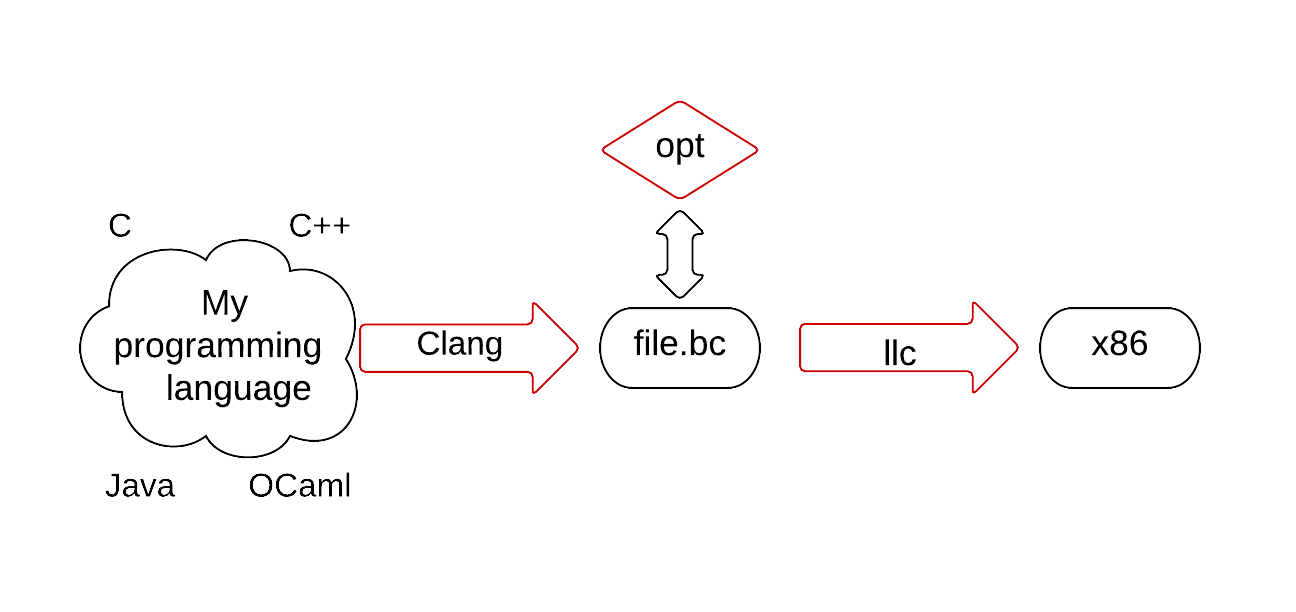
\includegraphics[width=0.5\textwidth]{llvmintro.PNG}
	\caption{Global view of LLVM use}
	\label{fig:llvmUse}
\end{figure}

\paragraph{}
To understand how LLVM is the solution to our problem, it is important to first introduce the notion of ``LLVM pass``.

\subsection{LLVM Pass}

\paragraph{}
LLVM is the collection of libraries that are already implemented, ready-to-use by the developer that allow code analyses and optimizations. Each analyse or optimization is call a pass. 

\paragraph{}
Concrete examples of pass already implemented by LLVM are :
\begin{itemize}
\item Memory allocation:This optimization consists in mapping memory slots into variables. This is helpful because it prevents the compiler to do constant memory access.
\item Constant propagation:This optimization consists in substituing the values of known constants in expressions directly during compilation.
\item Common subexpression elimination:This optimization consists in looking for common expressions which produce the same result and then compute this common expression only once in the code.
\item Many other passes can be found in the website of LLVM \cite{bworld}
\end{itemize}

\paragraph{}
A pass can be run on a complet code or only on a portion. This leads to the distinction of various types of pass. In our case, we will focuse on ModulePass (ran on the whole code) and FunctionPass (ran in functions)~\cite{LLVM:CGO04}.

\begin{comment}
\paragraph{}
What better than an example to illustrate how to implement and use a pass !\\

\subsubsection{2.2.1~~~~~~~LLVM Pass Example: Counting Machine Operations}
\begin{lstlisting}[language=Java, caption=Machine operation counting example, basicstyle=\scriptsize]
struct CountOp:public FunctionPass 
  {
    std::map<std::string, int> opCounter; 
    static char ID; CountOp() : FunctionPass(ID) {} 
    virtual bool runOnFunction(Function &F) 
    { 
      errs() << "Function " << F.getName() << "\n"; 
      for (Function::iterator bb = F.begin(), e = F.end(); 
      bb != e; ++bb) 
      {
        //errs() << "Name : " << bb.getName();
        for (BasicBlock::iterator i = bb->begin(), 
          e = bb->end(); i != e; ++i)
        {
          if(opCounter.find(i->getOpcodeName()) == 
            opCounter.end()) 
          {
            opCounter[i->getOpcodeName()] = 1; 
          } 
          else 
          {
            opCounter[i->getOpcodeName()] += 1; 
          }
          errs() << "\n";
        } 
      } 
      std::map <std::string, int>::iterator i = opCounter.begin(); 
      std::map <std::string, int>::iterator e = opCounter.end(); 
      while (i != e) 
      { 
        errs() << i->first << ": " << i->second << "\n"; i++; 
      } 
      errs() << "\n"; opCounter.clear(); return false;
     } 
  };
\end{lstlisting}

%Je vais aussi rajouter des mini bouts de code que je vais expliquer plus profondemment.
Let us take some time to explain how this code works:\\
\begin{itemize}
\item First of all, the pass is seen as a structure that inherit from FunctionPass class
\item In this structure, we define a map in which we will keep the result
\item We over-write the runOnFunction which will contain the analysis that has to be applied to the function F
\item We will loop on all basic blocks of the functions
\item For each basic block, we will loop on its instructions
\item For each instructions, we check if we already encounter it
\begin{itemize}
\item If it is the first time, we create it in the map
\item If not, we loop for it in the map and increase its appearence
\end{itemize}
\item Once the 2 loops are done, we printout the results
\end{itemize}


\subsubsection{2.2.2~~~~~~~LLVM Pass Save And Invoke: Pass Manager}
\paragraph{}
Once the pass is writting, it is time to compile it and use it. To do so, there are two steps to follow:
\begin{enumerate}
\item Save the pass in the Pass Manager: To be able to use the pass, it must be saved in the Pass Manager which contains all the passes implemented so far. For that purpose, it is mandatory to add the following lines of code inside the file containing the code for the pass:\\
\begin{lstlisting}[language=Java, caption=Pass saving, basicstyle=\scriptsize]
static RegisterPass<CountOp>X
("opCounter","Counts opcodes per functions") ;
\end{lstlisting}

\item Invoke the pass on a file: Once the pass is saved and the bytecode file is generated (Look in section 2.1), the following commands are used to invoke a pass:\\
\begin{lstlisting}[language=command.com, caption=Pass invoking, basicstyle=\scriptsize]
clang -c -emit-llvm file.c -o file.bc;
opt -load CountOp.so -opCounter -disable-output file.bc;
\end{lstlisting}
\end{enumerate}

\end{comment}

\begin{comment}
\subsubsection{2.2.3~~~~~~~LLVM Pass Chaining}

\paragraph{}
If each pass can produce a result, an analysis or perform an optimization, it is also possible to make different passes communicate. Indeed, it may occure that we need an analysis of the code (which is provided by a pass) in order to perform an optimization. To do so, the functions getAnalysisUsage and getAnalysis are used.

\paragraph{}
Let us illustrate this with an example: Counting the number of basic blocks in loops. The main challenge here is first to find where the loops are located in a code. And then, given these loops, count the number of basic blocks inside them.

\begin{lstlisting}[language=Java, caption=Pass chaining, basicstyle=\scriptsize]
void countBlocksInLoop(Loop *L, unsigned nesting) 
{
    unsigned numBlocks = 0;
    Loop::block_iterator bb;
    for(bb = L‐>block_begin(); bb != L‐>block_end();++bb)
        numBlocks++;
    errs() << "Loop level " << nesting << " has " 
    << numBlocks << " blocks\n";
    vector<Loop*> subLoops = L‐>getSubLoops();
    Loop::iterator j, f;
    for (j = subLoops.begin(), f = subLoops.end(); 
    j != f; ++j)
    {
        countBlocksInLoop(*j, nesting + 1);
    }
    
    virtual bool runOnFunction(Function &F) 
    {
    LoopInfo &LI = getAnalysis<LoopInfo>();
    errs() << "Function " << F.getName() + "\n";
    for (LoopInfo::iterator i = LI.begin(), e = LI.end();
    i != e; ++i)
        countBlocksInLoop(*i, 0);
    return(false);
}
\end{lstlisting}

\paragraph{}
As we can see in the code, in the runOnFunction, we run the LoopInfo pass, get the generated analysis thanks to getAnalysis and then on each loop of the result, run the countBlocksInLoop pass.
\end{comment}

%%%%%%%%%%%%%%%%%%%%%%%%%%%%%%%%%%%%%%%%%%%%%%%%%%%%%%%%%%%%%%%%%%%%%%%%%%%%%%%%
%%%%%%%%%%%%%%%%%%%%%%%%%%%%%%%%%%%%%%%%%%%%%%%%%%%%%%%%%%%%%%%%%%%%%%%%%%%%%%%%

\section{Open Computing Language: Open Standard For Parallel Programming}

\paragraph{}
To be able to write testing structures concerning OpenCl, a small explanation concerning OpenCL, the memory sharing representation and programming is advised \cite{stoneopencl}.


\subsection{Purpose And Definition}

\paragraph{}
Open Computing Language (OpenCL) is a framework dedicated to writting C programs that will be executed across multiple heterogeneous platforms (mainly composed of CPUs and GPUs). These platforms are represented as a number of \textbf{compute devices}. Each compute device will execute program, that is called \textbf{kernels}.
\begin{itemize}
\item One kernel can be executed in different compute devices
\item One compute device is composed of many processing elements
\end{itemize}

\paragraph{}
OpenCL programs are compiled at runtime. As said previously, the kernels are written in C, but to be more precise, it is a C version adapted to the device model.

\subsection{Structure Of OpenCL}

\paragraph{}
There are four different types of memory systems supported by devices:\begin{enumerate}
\item Global memory which corresponds to each device RAM
\item Constant memory which is a cached global memory
\item Shared local memory which can be accessed by processing elements of the same compute device.
\item Private memory accessible within one and only one processing element.
\end{enumerate}

\paragraph{}
In an OpenCL program, many initialisations must be done before actually running a kernel on compute devices. 
\begin{itemize}
\item We must create a context
\item Create a command queue in which we will store the kernels that need to be applied for each compute device.
\item Allocate the buffer memory objects that will act as memory for compute device.
\item Build the compute program
\item Build the compute program executable
\item Create kernel arguments (such as size, type, flags ...)
\item Enqueue command in the command queue
\end{itemize}

\begin{figure}[h]
	\centering
	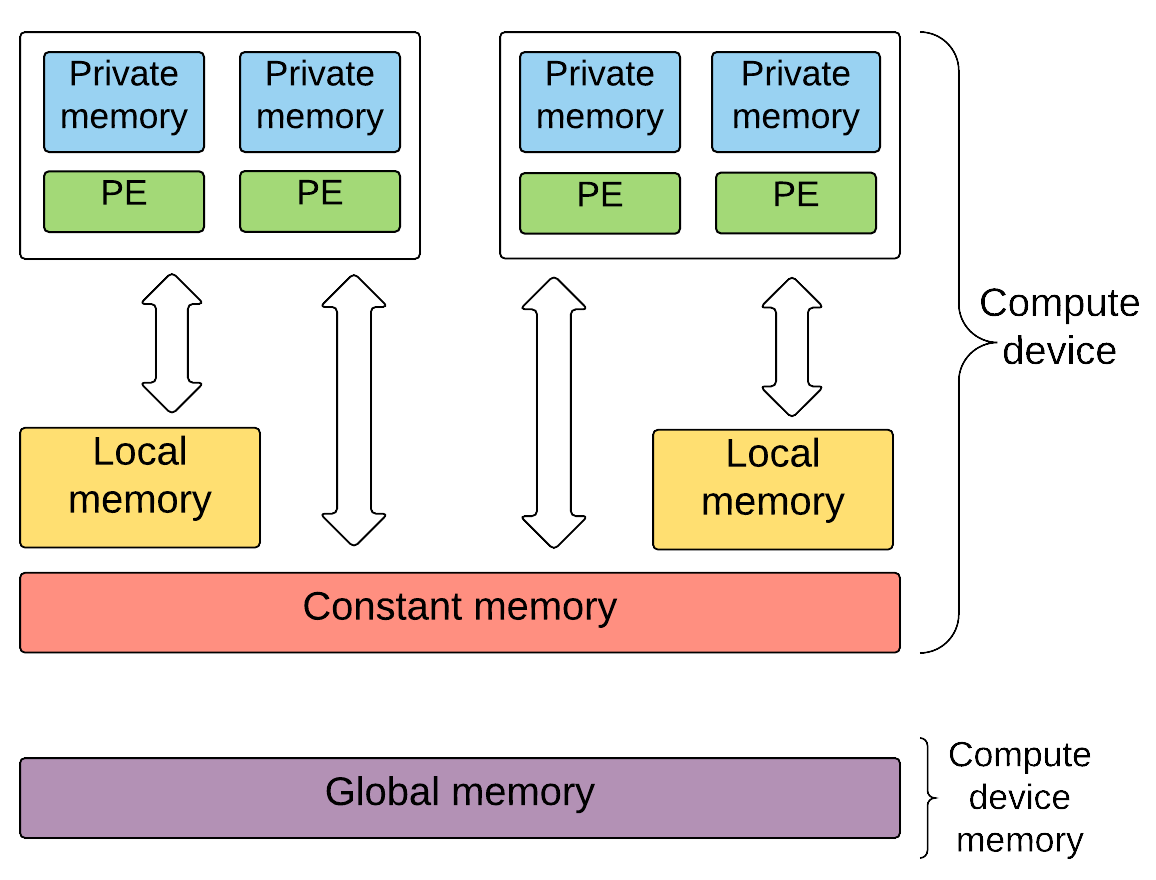
\includegraphics[width=0.5\textwidth]{mem.png}
	\caption{Example of out-of-bound memory access}
	\label{fig:mem}
\end{figure}

\paragraph{}
In our case, we must be able to change the way that OpenCL builds the program. We must be able to find a way to take the OpenCL code, generate a bytecode file that will be modified directly by LLVM. Then, the resulting bytecode is going to be given to OpenCL and execute it. 

\paragraph{}
For that purpose, when the building an executable comes, the bytecode generated by LLVM after passes will be used to build the final program.

\subsection{From Runtime to Compile Time}

\paragraph{}
For our work, we will need information concerning the kernels (such as size, access) to be able to perform test during memory access inside kernel functions. This information are only know during runtime. There for, we will need to find a way to communicate this information.

%%%%%%%%%%%%%%%%%%%%%%%%%%%%%%%%%%%%%%%%%%%%%%%%%%%%%%%%%%%%%%%%%%%%%%%%%%%%%%
%%%%%%%%%%%%%%%%%%%%%%%%%%%%%%%%%%%%%%%%%%%%%%%%%%%%%%%%%%%%%%%%%%%%%%%%%%%%%%
%%%%%%%%%%%%%%%%%%%%%%%%%%%%%%%%%%%%%%%%%%%%%%%%%%%%%%%%%%%%%%%%%%%%%%%%%%%%%%

\section{Memory Management Done By LLVM On OpenCl}

\paragraph{}
As a reminder, the goal was to create a tool that would give us as many information as possible concerning the buffers usage in an OpenCl program. Mainly, here are the steps to get this information:
\begin{enumerate}
\item First, we compile the OpenCl thanks to CLANG and LLVM to get a bytecode. In this step, we needed an intermediate tool that would help this generation. Here inters SPIR. SPIR (or Standard Portable Intermediate Representation) is the first intermediate language for representing parallel compute and graphics. Thanks to this tool, the generation of the bytecode from the OpenCL using LLVM is possible.
\item The generated bytecode is used in LLVM where a pass is applied to gather all type of memory management information (read, write).
\item Then, thanks to additional information, the pass will apply test concerning all memory access
\item Print this information to the developer in a structured way.
\end{enumerate}

\paragraph{}
To make the collection of information about memory usage possible,further material concerning the buffer used is needed. The first one is their size. Indeed, with the size given, it is possible to check for aliasing or out-of-bound memory access. To get this information, two solutions are offered to us:
\begin{enumerate}
\item Force the developer to give as arguments the sizes of used buffers in each function using them.
\item Create a LLVM pass that would change the signature of each function using the buffers dynamically by adding the sizes as arguments. Then, the bytecode generated after this pass is going to be passed to OpenCl so that the sizes needed are incorporated to the code. And all this would be made in compile time.
\end{enumerate}

\paragraph{}
The second option makes it all easier for the developer. First of all, he doesn't need to know that buffer sizes must be given. Second, if in the future, complementary information are needed for some reasons, no need to change all the structure of the functions. A LLVM pass is run to add other arguments for the needed information. The fact that the developer doesn't have to do more work highlights again the power of LLVM. A very important remark is that all this arguments adding and information passing is done in compile time.
Let us see in deep how each step in implemented.

%\subsection{From a OpenCl file to a bytecode file using LLVM/SPIR}

\subsection{Adding Arguments In The Bytecode Using LLVM}

\paragraph{}
In this step, the bytecode is generated from the OpenCL file using SPIR and LLVM. The goal is to modify this bytecode such that we have as many arguments as needed for additional information. In this case, let us consider the sizes of buffer used. So the first step is going to parse the code, and at each function declaration, we have to look for how many buffers are present as arguments. Then, we will add as many arguments. For that purpos,LLVM adds arguments of type Integer which name are "size\_" followed by the name of the buffer.\\   
It is important to notice that in LLVM, as we are looping inside the code, it is impossible to modify directly the function that we are manipulating. Therefore, the technique used is simple: We create a clone function that will have the same name, the same body. The difference between the old function and the clone is the number of arguments.

\begin{remark}
As we loop on the whole code, our pass is a ModulePass.
\end{remark}

\paragraph{}
The pass is structured as following:
\begin{enumerate}
\item First, we collect all function declaration inside the bytecode.
\item Then, we loop on the arguments of each function and look for usage of buffers. To do so, LLVM can give us the type of values. So we first look for declaration of pointers, and then we look for the ones which address space is equal to 1. Let us assume that the number of arguments that must be added is N.
\item Now, we get the type of the old function, and to this one we will add N arguments of type Integer, representing the sizes we need to add.
\item Then, we have to create the new clone function type to which we need to attach the body of the old function. The name of the clone function is the same as the old one.
\item Now we need to take the arguments names of the old function and map them to the arguments of the new function. Don't forget that we also need to rename the freshly N new added arguments. As a convention, we decided that, if we use a buffer name "x", then the added argument's name would be "size\_x".
\item The two last steps are to, first clone the old function into the new one. This will attach the new function to the current module. And then, we will have to delete the old function from the current module. 

%\begin{lstlisting}[language=Java, caption=Function cloning in LLVM, basicstyle=\scriptsize]
%SmallVector<ReturnInst*, 5> returns;
%llvm::CloneFunctionInto(clone, fn,
%                        VMap,
%                        false,
%                        returns,
%                        "");
%\end{lstlisting}
\end{enumerate}

\subsection{Inserting Complementary Information}

\paragraph{}
Now that the arguments are added inside the function's signture, there is another information that needs to be added inside the bytecode: Metadata.

\paragraph{}
Indeed, when OpenCL receives the freshly changed function, it will look inside the metadata to look for additional information. Basically, there are 5 types of information:
\begin{enumerate}
\item What is the address space of each argument of each function: 0 if private, 1 if global.
\item What is the qualification of each argument: If any argument is declared as a constant or not.
\item What is the type of each argument of each function.
\item What is the type qualification of each argument of each function.
\item What is the base type of each argument of each function.
\end{enumerate}
\paragraph{}
So actually, after adding the size argument, more metadata must be added. To do so, we will just create a new namedMDNode in which we insert the previous medata and just add metada concerning the added argument (sizes of buffers).
~Technically, if we added N arguments representing the size, we add N metada in each type of information.
\paragraph{}
In our case, if we added N arguments representing the sizes, we will add: 
\begin{itemize}
\item Their address space the number 0
\item Their access qualification is none
\item Their type is int
\item Their type qualification is none
\item Their base type is int
\end{itemize}


\subsection{Testing All Memory Access}
\paragraph{}
Once all requiered information (argument and metadata) is inserted, it is time to create tests. It has been decided that the most easy and mainstream test is aliasing. Indeed, knowing if two kernel buffers alias each other is easy just by having the address of the buffers and their sizes. Then, it is possible to know if address access are out of bound.

\paragraph{}
The way to perform test during compile-time is going to be done thanks to IRBuilder. Actually, we are adding instructions containing the tests we want to perform inside the bytecode. To do so, we use a IRBuilder that allows us creating if/then/else instructions, also known as IcmpInst. IRBuilder is a LLVM class that allows the user to create nearly anything possible. 

\subsubsection{Aliasing}
Aliasing it the fact that a data location in memory can be accessed through different symbolic names in the program. Let us have an example: 
\begin{figure}[h]
	\centering
	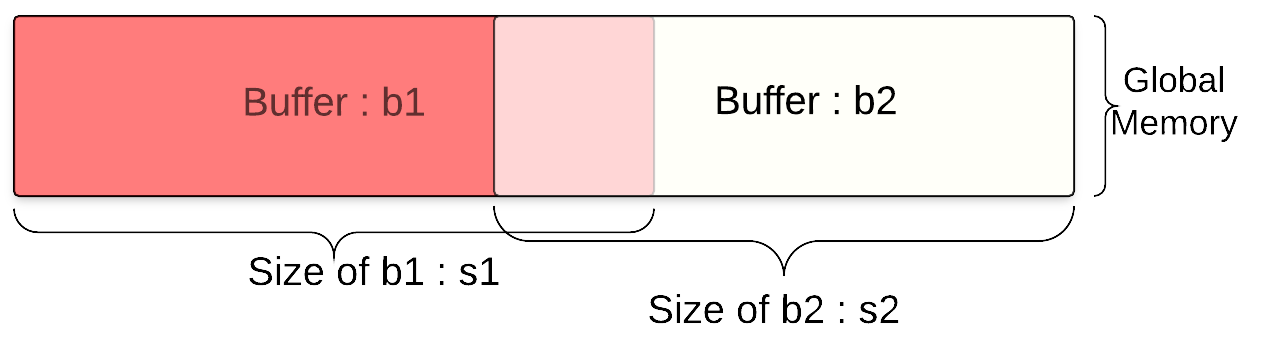
\includegraphics[width=0.5\textwidth]{alias.png}
	\caption{Example of memory aliasing}
	\label{fig:alias}
\end{figure}

\paragraph{}
In this case, we can see that the base pointer of buffer b2 is located inside the buffer b1. The major problem in this case is the following: if any one reads in the aliasing location (represented in pink in \ref{fig:OFB}) and that someone else writes in it, this leads to major memory error. The one who reads before a write doesn't have the update version. 

\paragraph{}
The algorithm used so detect aliasing used in this work is the following: \\
\begin{algorithm}[H]
\SetAlgoLined
\KwResult{Return true if alias; else return false }
    List listOfKernels; List listOfSizes\;
    Kernel currentK = listOfKernels[0]\;
    Size currentS   = listOfSizes[0];
    i = 1\;
 \While{i \neq listOfKernels.size~}
 {
  \eIf{currentK \textless ~ listOfKernels[i]~}
  {
   \eIf{ (currentK + currentS) \textless ~ listOfKernels[i]~}
   {
    No Alias;  return false\;
   }
   {
    Alias; return true\;
   }
  }
  {
  \eIf{listOfKernels[i] \textless ~ currentK}
  {
   \eIf{ (listOfKernels[i] + listOfSizes[i]) \textless ~ currentK}
   {
    No Alias;  return false\;
   }
   {
    Alias; return true\;
   }
  }
  }
 }
 \caption{Detecting aliases}
\end{algorithm}
\paragraph{}
So the main idea is to do computation on kernel buffer's addresses and sizes.

\subsubsection{Out Of Bound}
\paragraph{}
Out-of-bound memory access happens when a load or store instruction is executed and that the program tries to access to a memory space that either doesn't exist or to a memory space that is forbidden.
To explain the algorithm used, let us base ourselves on the figure 

\begin{figure}[h]
	\centering
	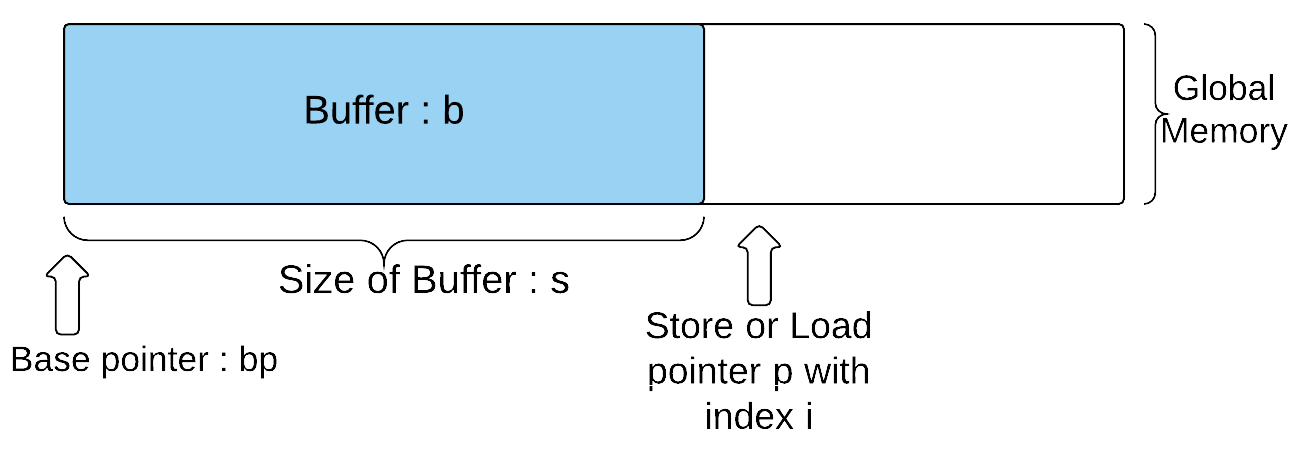
\includegraphics[width=0.5\textwidth]{OFB.png}
	\caption{Example of out-of-bound memory access}
	\label{fig:OFB}
\end{figure}

\paragraph{}
Knowing if there is any out-of-bound memory access needs to be done the following way: 
\begin{itemize}
\item Get the list of kernel buffers and sizes of a function
\item Get the list of load instructions and store instructions of a function
\item For each of these instructions, we retrieve the pointer p and the index i then extract the base pointer bp from it. Then, we look in our list of defined kernels this base pointer. 
    \begin{enumerate}
    \item If the base pointer computed doesn't correspond to any kernel address pointer of the kernel list, then the memory access is totally false. 
    \item If the sum of the pointer base and the index is greater than the kernel's address and its size, than we are performing an out-of-bound memory access (as in our figure \ref{fig:OFB}
    \item Else, the memory access can be done.
    \end{enumerate}
\end{itemize}

\paragraph{}
\begin{remark}
After adding argument and test instructions, the bytecode has been modified. Therefore, it is mandatory to return true at the end of the pass to notify to other passes the modification.
\end{remark}

%%%%%%%%%%%%%%%%%%%%%%%%%%%%%%%%%%%%%%%%%%%%%%%%%%%%%%%%%%%%%%%%%%%%%%%%%%%%%%
%%%%%%%%%%%%%%%%%%%%%%%%%%%%%%%%%%%%%%%%%%%%%%%%%%%%%%%%%%%%%%%%%%%%%%%%%%%%%%
%%%%%%%%%%%%%%%%%%%%%%%%%%%%%%%%%%%%%%%%%%%%%%%%%%%%%%%%%%%%%%%%%%%%%%%%%%%%%%

\section{Conclusion}

\paragraph{}
In this paper we presented a way to do memory management on OpenCL code directly at compile time thanks to SPIR. The program has been tested on simple OpenCl code. During the work, assumptions had to be made and we took care of basic coding. 

\subsection{Future Work}

\paragraph{}
There are many improvements that can be made: 
\begin{itemize}
\item During the work, we made the following assumption: inside the kernel function that needs to be modified (adding argument and tests), if there is any call to other functions using kernel buffers, we will need to change this call instruction by adding again the argument directly inside the call.
\item Another test that can be added is flag testing. Indeed, the kernel buffers have different access rights. They can be in write only, read only or read/write. This information can also be found during runtime. As for the size, we can test all access (load or store instruction) to the kernel buffer, and see if they don't violate the access right to each kernel.
\item We can also add a test concerning concurrent access of a part of a local memory. At this point, the notion of DMA (direct memory access) race is introduced. 
\end{itemize}

\subsection{Application}
\paragraph{}
This tool has been explicitly created to overcome memory management problem. Indeed, we get enough information to be aware of aliasing or out-of-bound memory access. The next big step would be detecting DMA races. Thanks to the possibility to create testing structures directly inside the bytecode, this can be done and help OpenCL programmers write more secure and more powerful code. 

%%%%%%%%%%%%%%%%%%%%%%%%%%%%%%%%%%%%%%%%%%%%%%%%%%%%%%%%%%%%%%%%%%%%%%%%%%%%%%
%%%%%%%%%%%%%%%%%%%%%%%%%%%%%%%%%%%%%%%%%%%%%%%%%%%%%%%%%%%%%%%%%%%%%%%%%%%%%%
%%%%%%%%%%%%%%%%%%%%%%%%%%%%%%%%%%%%%%%%%%%%%%%%%%%%%%%%%%%%%%%%%%%%%%%%%%%%%%

\section{Acknowledgments}

\paragraph{}
First, I would like to thank my supervisor Ylies Falcone for proposing me this work and guiding me the whole time. A great thank you to Jean-Fran\c{c}ois Mehaut who gave me good advices during the work. I would like to show my gratitude to Brice Videau, who helped me a lot in the realization of this project and gave me precious remarks. Without his guidance, this work wouldn't be what it is.

\paragraph{}
I would also like to sincerely thank the INRIA Corse team for sharing their huge knowledge of LLVM programming. A special thank you to Fabian Grubber for his insights and very useful help during coding passes.

\appendix

\nocite{leestatic}
\nocite{test:test}
\nocite{LLVM:CGO04}
\nocite{LattnerAdve:tutorial}
\nocite{fabeiro2013ocloptimizer}
\nocite{collingbourne2012symbolic}
\nocite{lattner2004llvm}
\nocite{moll2014bounds}
\nocite{43308}
\nocite{threadsanitizer}
\nocite{bworld}
\nocite{stoneopencl}

%% The file named.bst is a bibliography style file for BibTeX 0.99c
\bibliographystyle{unsrt}
\bibliography{ijcai11}

\end{document}

